\section{Continuation screen and model-assisted preparation}
\label{sec:model-followup}
\textbf{Status: four physical engineering trials complete; CPU model fails qualification.}
These separate investigations change no original candidate, objective or checking
result. The physical screen tests a composition hypothesis on one exposed case;
the learned model and action-changing filter remain undeployed.

\subsection{Prospectively frozen continuation method}
Before original independent checking, we froze random-search draw 2 from generation
one, task 0019/base and exposed seed 6101920. Its earlier factual closure at 482
motivates this engineering case. All four references share that selected matrix
and development information: native only, closure only, fixed-clock handoff and
privileged supported-closure handoff. This tests feasibility, without a fresh-seed
generalization or EA claim. The clock adds elapsed-query information beyond the
original 44 actor coordinates; privileged gating additionally uses monitor labels.

The privileged trigger requires three consecutive post-control observations with
closed lid, support and no preceding violation. Observation zero is excluded.
Loss of qualification before the next eight-control query cancels the trigger.
Switch there and latch native execution, preserving the policy Gaussian stream,
episode identity and seed. The fixed clock is 488 from the exposed example.
Native and closure-only references make no switch. Every condition retains the
same encoder schedule, native termination and full 2,000-control horizon.

The four-total-start cap includes partial failures, with no automatic replacement
or extra decoder probe. Each start has independent startup/full-wall guardians,
durable admission and exclusive policy-service ownership. Original60 completion,
full restoration, unchanged source and fresh machine/rate/armed-clock/capacity
checks passed before dispatch. The compound reader verifies actual components,
RNG continuity, executed commands, exact native monitor entries and captured
server returns. Software preparation used 74 synthetic sampler calls, separately
from the 368 neural decoder-only calls.

A later stage requires a positive closure prefix and actual native continuation,
no whole-episode violation, and a new ordered holding/lift/transport milestone
strictly after switching or first safe requested completion after switching.
At-switch observations belong to the prefix. Holding uses the native predicate
without an independent body-link grasp witness. This criterion authorizes no
automatic extra starts; none of the actual references meets it.

\subsection{Completed physical screen}
All four starts reach 2,000 controls and pass full verification, with no invalid
start (Table~\ref{tab:screen}). No requested/raw goal or native holding occurs.
Native never contacts the target. Closure-only contacts it and first closes at
observation 596, remaining nonviolating with 1,405 closed observations, without
holding. This repeats partial closure on the selected exposed seed.

\begin{table*}[t]
\caption{Separate engineering screen: one full trial per mode, on the same exposed
task/seed. SC/UC and SU/UU are requested completion/safety categories; $V$ is the
whole-episode violation. Stage is the highest ordered milestone before any
violation; stage 1 is supported closure. $A_{\rm post}$ counts actual native
controls after a switch; native-only has no switch and executes 2,000 native
controls. $t_V$ is the first violating observation; $N_{\rm close}$ counts executed
closing inputs. These four cases establish no rate, causal effect or transfer.}
\label{tab:screen}
\begin{tabular}{lrrrrrrrrrr}
\toprule
Mode & SC & UC & SU & UU & $V$ & Stage & Switch & $A_{\rm post}$ & $t_V$ & $N_{\rm close}$ \\
\midrule
Native & 0 & 0 & 1 & 0 & 0 & 0 & n/a & 0 & n/a & 0 \\
Closure-only & 0 & 0 & 1 & 0 & 0 & 1 & n/a & 0 & n/a & 0 \\
Clock handoff & 0 & 0 & 0 & 1 & 1 & 0 & 488 & 1512 & 475 & 40 \\
Privileged handoff & 0 & 0 & 0 & 1 & 1 & 1 & 448 & 1552 & 471 & 142 \\
\bottomrule
\end{tabular}
\end{table*}

Clock execution loses uprightness while still supported and open at observation
475, before switching at 488. Its later first closure at 531 follows that
violation and earns no safe ordered credit. Privileged execution closes at 445,
debounces at 447 and switches at 448. It loses uprightness at observation 471,
23 native controls later, while still closed and supported. These timings do
not identify an action-specific cause; clock's first violation cannot be
attributed to its later handoff. Neither trial adds ordered holding, lift or
transport. There is no late native-goal confirmation to satisfy the alternative
completion-after-switch criterion. The screen is not expanded.

\begin{figure*}[t]
\centering
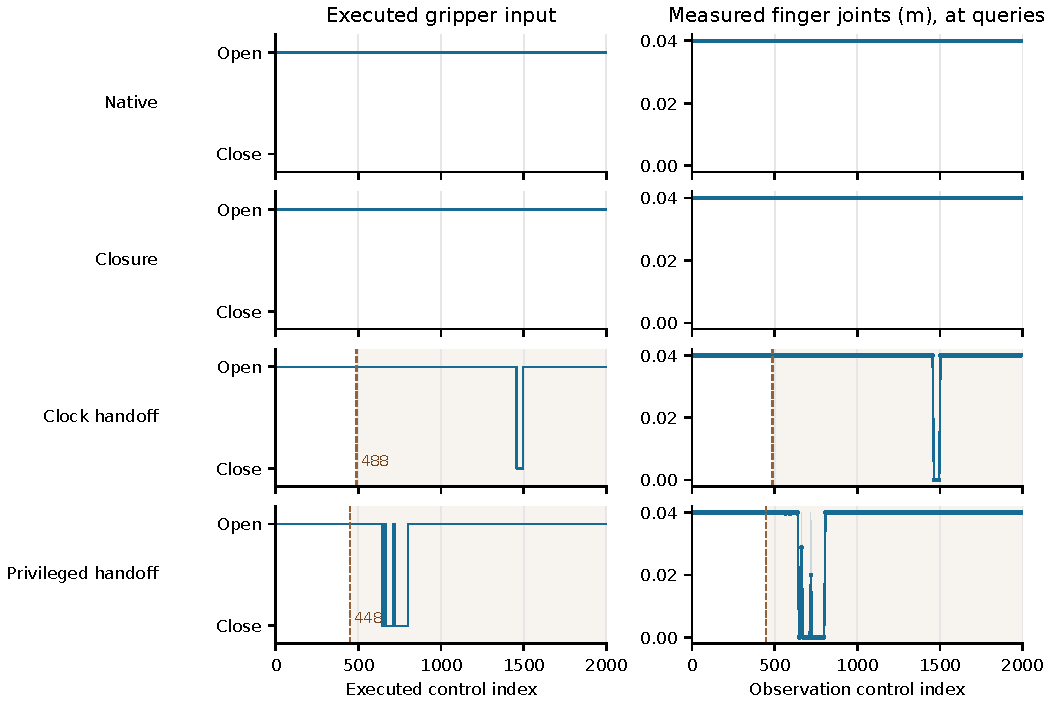
\includegraphics[width=\textwidth]{../../figures/ManiGuard/continuation-screen-20261020/gripper-trajectories.pdf}
\caption{Actual gripper inputs and measured query-time finger joints in the four
completed engineering trials. Dashed lines mark actual switches; tan regions
show native continuation. At-switch positions precede the first native action.
Points are two-joint means and blue bands span the two joints, without implying
uncertainty, fingertip aperture or a body-link grasp. A closing input does not
prove holding. Every plotted trace is bound to the completed physical audit.}
\Description{Native and closure-only command opening throughout. Both handoffs
later command closing and reach near-zero finger joints, without native holding.}
\label{fig:screen-gripper}
\end{figure*}

Native and closure-only command opening throughout, with finger joints near
.04 m. The handoffs issue 40/142 closing inputs, first at control 1456/642,
respectively, after their first violations. Measured joints later reach
approximately zero, and native holding remains absent
(Figure~\ref{fig:screen-gripper}). The observed failures therefore require more
than an account of uniformly opening commands. Closure timing also differs
across nominally matched streams. Unequal initial camera images and the single
selected case limit causal interpretation; full reset-state identity is unproven.
A timeout does not establish
irreversibility or a unique perception, dynamics or controller defect.

This screen adds 8,000 controls, 1,000 physical policy requests, 8,040 returned
environment steps, 48,356 known physics ticks and 2,000 encoder images. Across
both protocols and all engineering attempts, totals are 120,131 controls,
15,019 physical policy requests plus 368 decoder-only requests, 726,749 known
physics ticks and 30,038 encoder images. All 15,387 neural-policy returns
reconcile exactly; all nine original service prefixes remain unchanged. At the
dated 16:57 UTC allocation snapshot, both GPUs account for 43.179 allocated
GPU-hours and a \$13.226 upper-bound estimate, without verified billing or final
rental closure. Later preservation time remains additional.

\subsection{CPU model audit and rejected deployment}
A five-member episode-bootstrap ridge ensemble predicts the next 44 compact
features from 153 inputs: current/previous features, a history-valid flag and
eight executed eight-dimensional commands. It uses 32 fixed nonlinear random
features and separate heads for a new violation and five task predicates.
Actual-future-feature readouts distinguish readout error from imagined-dynamics
error. The model generates no future RGB or complete closed-loop VLA episode.
Prepared residual/filter, candidate-allocation and ROSARL interfaces are CPU
prototypes. ROSARL needs a declared external value estimator and frozen practical
penalty~\cite{rosarl}; there is no trained ROSARL task-policy baseline here.
World-model safety planning already has precedents~\cite{safedreamer}.

The audit was frozen before fitting. Eight shared-initial episodes on tasks
0019/0009 supply 1,992 fitting transitions; development tasks 0017/0013 supply
249 calibration and 83 diagnostic transitions. Splits are by whole exposed task,
without checking outcomes. Their 18,666 original acquisition controls are reused,
without being charged again. Risk fitting excludes already-doomed prefixes.

\begin{table}[t]
\caption{CPU prediction audit on one diagnostic episode. RMSE rows are correlated
within that episode. The frozen model/persistence ratio gate is at most .90 in
every block; all three fail.}
\label{tab:model-audit}
\begin{tabular}{lrrr}
\toprule
Feature block & Model & Persistence & Ratio \\
\midrule
Robot/history & .16805 & .08516 & 1.973 \\
Overview & .04381 & .02848 & 1.538 \\
Wrist & .06380 & .05481 & 1.164 \\
\bottomrule
\end{tabular}
\end{table}

Actual-feature readout MAE is .191 for closure, .209 for holding, .662 for
uprightness and .210 for support, above the .10 gate. Fitting has positive
closure/holding in only one episode each, no in-goal positive episode or safe
completion; its observed closure follows a violation. Calibration has one episode
against the required minimum 20. Conservative abstention rejects every prefix;
its 100\% negative-prefix alarm rate is not a qualified classifier's false-alarm
rate. Counterfactual-action coverage remains unsupported. The audit costs 27,412
training-row uses and 5,395 model-head row queries, with no new physical controls,
VLA calls or encoder images. It is not refitted on the four new screen trials.
The failed model remains excluded from physical action selection.
